
\documentclass[twoside,twocolumn]{article}
\usepackage{datetime}
\usepackage{blindtext} % Package to generate dummy text throughout this template 
\usepackage{graphicx,floatrow}

\usepackage[sc]{mathpazo} % Use the Palatino font
\usepackage[T1]{fontenc} % Use 8-bit encoding that has 256 glyphs
\linespread{1.05} % Line spacing - Palatino needs more space between lines
\usepackage{microtype} % Slightly tweak font spacing for aesthetics

\usepackage[english]{babel} % Language hyphenation and typographical rules

\usepackage[hmarginratio=1:1,top=32mm,columnsep=20pt]{geometry} % Document margins
\usepackage[hang, small,labelfont=bf,up,textfont=it,up]{caption} % Custom captions under/above floats in tables or figures
\usepackage{booktabs} % Horizontal rules in tables

\usepackage{lettrine} % The lettrine is the first enlarged letter at the beginning of the text

\usepackage{enumitem} % Customized lists
\setlist[itemize]{noitemsep} % Make itemize lists more compact

\usepackage{abstract} % Allows abstract customization
\renewcommand{\abstractnamefont}{\normalfont\bfseries} % Set the "Abstract" text to bold
\renewcommand{\abstracttextfont}{\normalfont\small\itshape} % Set the abstract itself to small italic text

\usepackage{titlesec} % Allows customization of titles
\renewcommand\thesection{\Roman{section}} % Roman numerals for the sections
\renewcommand\thesubsection{\roman{subsection}} % roman numerals for subsections
\titleformat{\section}[block]{\large\scshape\centering}{\thesection.}{1em}{} % Change the look of the section titles
\titleformat{\subsection}[block]{\large}{\thesubsection.}{1em}{} % Change the look of the section titles

\usepackage{fancyhdr} % Headers and footers
\pagestyle{fancy} % All pages have headers and footers
\fancyhead{} % Blank out the default header
\fancyfoot{} % Blank out the default footer
%\fancyhead[C]{Running title $\bullet$ May 2016 $\bullet$ Vol. XXI, No. 1} % Custom header text
\fancyfoot[RO,LE]{\thepage} % Custom footer text

\usepackage{titling} % Customizing the title section

\usepackage{hyperref} % For hyperlinks in the PDF

%----------------------------------------------------------------------------------------
%	TITLE SECTION
%----------------------------------------------------------------------------------------

\setlength{\droptitle}{-4\baselineskip} % Move the title up

\pretitle{\begin{center}\Huge\bfseries} % Article title formatting
\posttitle{\end{center}} % Article title closing formatting
\title{Implementing MAXQ and Qlearning methods in R and applying them to the taxi problem \thanks{Reinforcement learning undergraduate class project}}% Article title
\author{%
\textsc{Mihai Groza} \\[1ex] % Your name
\normalsize Concordia University \\ % Your institution
\normalsize \href{mailto:fill this}{fill this} % Your email address
\and % Uncomment if 2 authors are required, duplicate these 4 lines if more
\textsc{Khaled Fouda} \\[1ex] % Second author's name
\normalsize Concordia University \\ % Second author's institution
\normalsize \href{mailto:khaledsfouda@gmail.com}{khaledsfouda@gmail.com} % Second author's email address
}

%\newdate{date}{02}{02}{2020}
%\date{\displaydate{date}}
%\date{\today} % Leave empty to omit a date
\renewcommand{\maketitlehookd}{%
\begin{abstract}
last thing to do.
\end{abstract}
}

%----------------------------------------------------------------------------------------

\begin{document}

% Print the title
\maketitle

%----------------------------------------------------------------------------------------
%	ARTICLE CONTENTS
%----------------------------------------------------------------------------------------

\section{Introduction}
later.
%------------------------------------------------
\section{Environment}
%\begin{center}
\begin{figure}
\centering
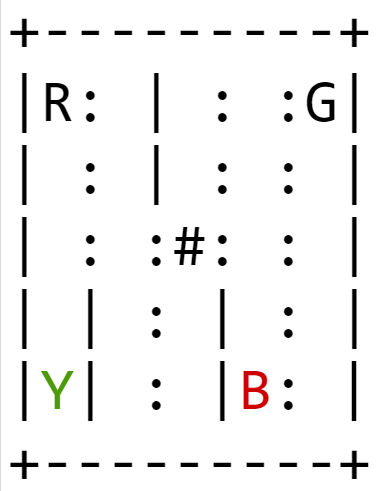
\includegraphics[scale=.4]{taxi.png} 
\caption{generated by render(s)}
\end{figure}
%\end{center}
The taxi's - shown as \# - goal is to first pick up the passenger from one of the four places (R,Y,G,B) where the current location of the passenger is shown in green. After picking up the customer, the next and final goal is to drive him to his destination which is one of the four places (R,Y,G,B) and the destination is shown in red.\\

The state is defined as a set (taxi\_row, taxi\_column, passenger\_location, destination\_location) where:\\
taxi\_row and taxi\_column take values from 1 to 5 as we have 5x5 grid,\\
passenger\_location and destination\_location take values [1,2,3,4] for [R,Y,G,B], furthermore, if the passenger is in the taxi then they takes a location 5.\\
That being said, we have $5*5*5*4=500$  different states.\\

The set of actions available is ( North, South, East, Wast ) with ids 1 to 6.\\

If the taxi successfully dropped off the passenger then the episode is over and they receive a reward of +20, if they dropped the passenger at a wrong location or before picking them up first then they receive a reward of -10 and continue the episode to drop the passenger at the right location (ie. no change in the state). Similarly if they attempted to pick the passenger at the wrong place. Otherwise, they receive a reward of -1 for each step taken. Note that hitting the wall results in a reward of -1 and no change in the state.\\

I have implemented the following functions for the environment:\\
\begin{itemize}
\item render(state) : returns nothing and prints out the environment at the current state.\\

\item encode(s) : maps each state to an integer between 1 and 500.\\

\item decode(i): The inverse of encode(s). it takes an integer between 1 and 500 and returns the corresponding state.\\

\item loc.indx(i): maps the four pick/drop locations (1,2,3,4) to a (row,column) set.\\

\item hitting.wallQ(r,c,a): returns True if taking the action (a) at the location (r,c) would results in hitting the wall.\\

\item step(s,a) returns (s',r) at state s, it takes the action a, observes the reward r and the next state s' 
\end{itemize}
 
%-------------------------------------------------
\section{MAXQ method}


%------------------------------------------------
\section{Qlearning method}
\section{Results}
\section{Similar projects}
\section{Final thoughts}

%----------------------------------------------------------------------------------------
%	REFERENCE LIST
%----------------------------------------------------------------------------------------

\begin{thebibliography}{99} % Bibliography - this is intentionally simple in this template

\bibitem[Figueredo and Wolf, 2009]{Figueredo:2009dg}
Figueredo, A.~J. and Wolf, P. S.~A. (2009).
\newblock Assortative pairing and life history strategy - a cross-cultural
  study.
\newblock {\em Human Nature}, 20:317--330.
 
\end{thebibliography}

%----------------------------------------------------------------------------------------

\end{document}
